\section{Beispielseite: Reiseziele}
\label{bspreisen}
\textsc{Stefan Waidele}

\begin{figure}[h]
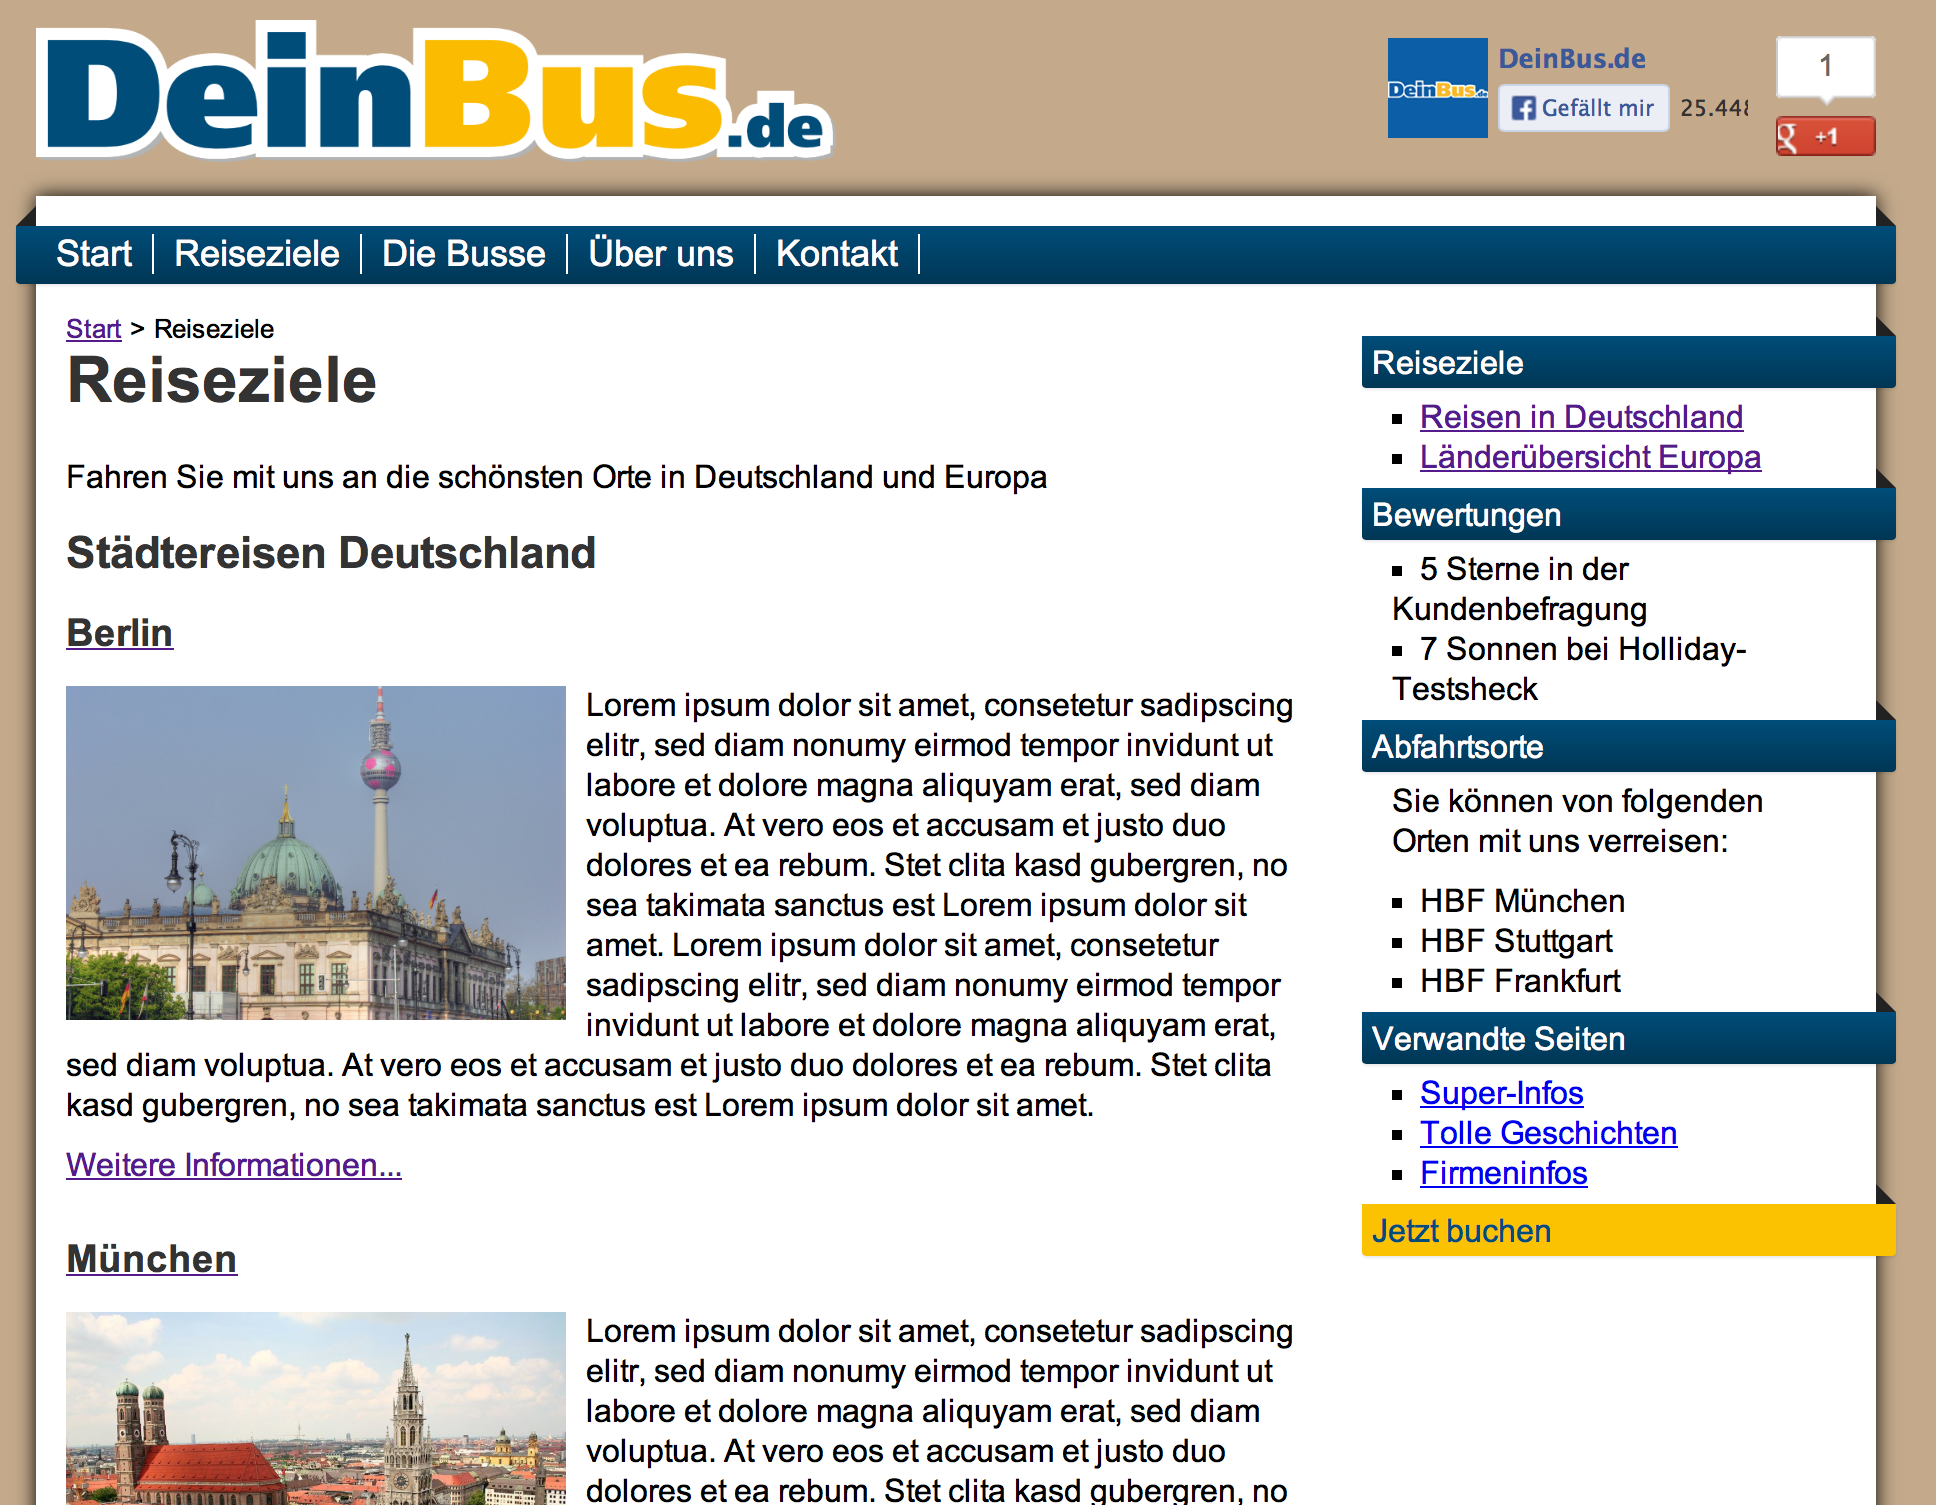
\includegraphics[width=\hsize]{scr_reisen}
\caption{Screenshot: �bersichtsseite Reisen}
\label{scr:reisen}
\end{figure}

Die Seite "`Reiseziele"' listet eine Auswahl der beliebtesten Reiseziele in Deutschland und Europa auf. 
Die nach L�ndern sortierten �bersichtsseiten sind hier in der Seitenleiste verlinkt. Die Seite wird 
von der Datei \code{/reiseziele/index.php} erzeugt.

Die hier gezeigten Elemente, besonders das Einbinden der gemeinsamen Elemente in \code{header.php} sowie \code{footer.php}
aber auch der individuelle Content--Bereich und die Seitenleite sind bei allen Seiten dieses Projekts gleich.

\subsection{Aufruf von header.php}

\begin{figure}[h]
\begin{minted}[bgcolor=bg]{php}
<?php 
$title="Reiseziele";
$desc = "�bersicht �ber unsere Reiseziele - Deutschland - Europa";
include($_SERVER['DOCUMENT_ROOT'].'/header.php'); 
?>
\end{minted}
\caption{Quellcode: Aufruf von header.php (PHP)}
\label{abb:header}
\end{figure}

Zun�chst werden hierin einige Angaben wie der Seitentitel in PHP-Variabeln abgelegt, um
dann die f�r alle Seiten gleiche Header-Datei \code{/header.php} aufzurufen (Vergleiche Abbildung~\ref{abb:header}). Hierin ist der gesamte HTML-Head Bereich 
sowie der f�r Besucher sichtbare Seitenkopf bis zum Navigationsmen� gespeichert. Der Ersteller oder Bearbeiter
der Reise�bersichtsseite braucht sich hierum nicht zu k�mmern.

\subsection{Realisierung der Breadcrumb--Navigation}

Nachdem die beiden f�r das Layout notwendigen DIVs ge�ffnet wurden, muss nun die Breadcrumb--Navigation angezeigt werden, anhand derer der Besucher schnell sehen kann, an welcher Stelle der Hierarchiestufe er sich befindet. Die zuvor besuchten, h�her liegenden Seiten sollen verlinkt sein. Der HTML--Code ist wie in Abbildung~\ref{abb:breadcrumb} zu gestalten. 

\begin{figure}[h]
\begin{minted}[bgcolor=bg]{html}
<div id="breadcrump">
   <a href="/" title="Zur�ck zur Startseite">Start</a> 
   > <a href="/reiseziele/" title="Kurz�bersicht">Reiseziele</a> 
   > Reisen in Deutschland
</div>
\end{minted}
\caption{Quellcode: Breadcrumb--Navigation (HTML)}
\label{abb:breadcrumb}
\end{figure}

\subsection{Kurzvorstellung der Reiseziele}

Nachdem der Seitentitel mit dem HTML-Tag \code{<h1>} und die Reiseregion (Deutschland bzw. Europa) mit \code{<h2>} ausgezeichnet wurden, beginnt die Beschreibung der eigentlichen Reiseziele mit einer �berschrift der Stufe \code{<h3>}, gefolgt von einem passenden Bild und dem beschreibenden Text. Am Ende der Kurzbeschreibung wird auf die Seite mit den entsprechenden Detailinformationen verlinkt. Somit ergibt sich eine Abfolge wie in  Abbildung~\ref{abb:stadt} zu sehen ist:

\begin{figure}[h]
\begin{minted}[bgcolor=bg]{html}
<div class="excerpt clearfix">
   <a href=""><h3>Berlin</h3></a>
   <a href=""><img src="/img/berlin1.jpg" 
                   alt="Fernsehturm in Berlin" /></a>
   <p>Lorem ipsum dolor sit amet, ...</p>
   <p><a href="">Weitere Informationen...</a></p>
</div>
\end{minted}
\caption{Quellcode: Reiseinformationen (HTML)}
\label{abb:stadt}
\end{figure}

Hierbei ist zu beachten, dass die Detailseite nicht nur am Ende des Textes, sondern auch bei der �berschrift und beim Bild verlinkt ist, um den Kunden m�glichst direkt zu den gew�nschten Informationen zu bringen.

Dieses Muster kann dann f�r jedes darzustellende Reiseziel wiederholt werden.
Aufgrund der Formatierungen im CSS muss der Redakteur wohl den korrekten HTML-Syntax sicherstellen, es befinden sich jedoch kaum Layout-Anweisungen im HTML-Code. Somit wird ein einheitliches Erscheinungsbild erzielt.

\subsection{Seitenleiste}

Auch die Seitenleiste wird in den entsprechenden Layout-DIVs nach einem einfachen, sich wiederholenden Muster realisiert.
Wie in Abbildung~\ref{abb:sidebar} zu erkennen ist, bestehen die �berschriften der Seitenleisten aus einem als \code{DIV} ausgezeichnetem Text, der von den Unterpunkten in Form einer HTML-Liste gefolgt wird. 

\begin{figure}[h]
\begin{minted}[bgcolor=bg]{html}
<div id="sidebar" class="clearfix">
   <div class="sidebar-topic">Reiseziele
   <span class="corner-right"></span></div>
      <ul>
         <li><a href="">Reisen in Deutschland</a></li>
         <li><a href="">L�nder�bersicht Europa</a></li>
      </ul>
   <div class="sidebar-topic">Bewertungen
   <span class="corner-right"></span></div>
      <ul>
         <li>5 Sterne in der Kundenbefragung</li>
         <li>7 Sonnen bei Holliday-Testsheck</li>
      </ul>
</div>
\end{minted}
\caption{Quellcode: Seitenleiste (HTML)}
\label{abb:sidebar}
\end{figure}

\subsection{Aufruf von footer.php}

Zum Abschluss der Seite wird mit der Codezeile aus Abbildung~\ref{abb:footer} noch die Datei \code{/footer.php} eingelesen. Hier wird der einheitliche Seitenfu� mit den Links zum Impressum, zu den AGBs und zur Sitemap dargestellt. 

\begin{figure}[h]
\begin{minted}[bgcolor=bg]{php}
<?php include($_SERVER['DOCUMENT_ROOT'].'/footer.php'); ?>
\end{minted}
\caption{Quellcode: Aufruf von footer.php (PHP)}
\label{abb:footer}
\end{figure}
\clearpage
